%=====================================================================
\section{Why \ember{} Misses Quiet Concepts}
\label{sec:motivation}
%=====================================================================

\begin{figure*}[t]
  \centering
  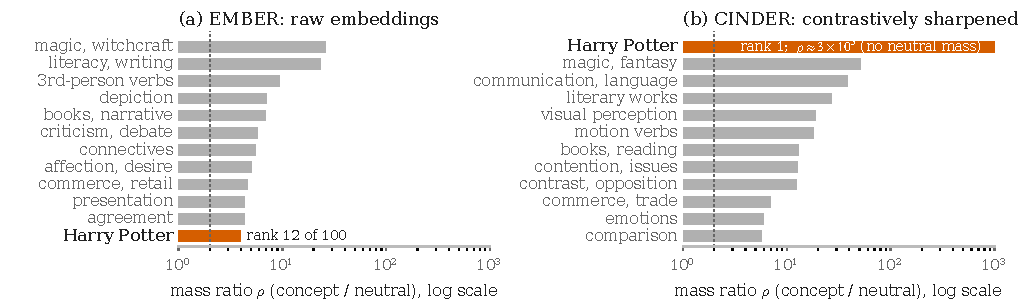
\includegraphics[width=\textwidth]{figures/hp_rho.pdf}
  \caption{Harry Potter is a quiet concept in \ember{}'s matrix and the strongest one after Contrastive Sharpening. Shown are the top 12 of 100 sparse-MF features for Harry Potter on Gemma-2-2B-it (seed 42), ranked by \ember{}'s mass ratio $\rho$ (Eq.~\ref{eq:rho}); labels paraphrase each feature's LLM description. (a)~On the raw embeddings, eleven generic topics outrank the concept feature. (b)~On the sharpened matrix, with the same 1\% row sparsity, the concept feature ranks first and has no neutral mass. The dotted line marks \ember{}'s threshold $\tau = 2$.}
  \label{fig:hp}
\end{figure*}

A natural question is how reliably \ember{}'s first two stages find the target concept.
To study this, we reproduced \ember{} on Gemma-2-2B-it, matching the published accuracies within four points (\S\ref{app:ember}), and inspected each stage on its flagship concept, Harry Potter, before testing each observation on more concepts and seeds.
We find five issues, summarized in Table~\ref{tab:diagnosis}.

\paragraph{The concept is a quiet direction}
Sparse MF minimizes the squared reconstruction error, so a feature is only as valuable to it as the energy it explains.
Intuitively, a topic shared by many tokens explains much of this energy, while a concept carried by a few dozen rare names explains little.
Figure~\ref{fig:hp}a shows the consequence for Harry Potter: eleven generic features, such as magic, writing, third-person verbs and books, score higher than the concept feature on \ember{}'s own concept ratio.
The cost appears in the feature's tail.
Its first 19 tokens all belong to Harry Potter, but only 2 of the next 11 do, and further down are Nestl\'e, Lego, Trump and Latin taxonomic suffixes, all of which \ember{} would edit (\S\ref{app:examples}).
We expect concepts to be quiet partly because their tokens are rare, and rare tokens receive fewer gradient updates during training \citep{gao2019representation}.
\pending{WP1: across 38 concepts, the energy rank of the concept direction in the raw matrix, and whether concept tokens are rarer and lower in variance.}

\paragraph{One width does not fit all concepts}
\ember{} keeps the top 1\% of tokens in every feature, 48 tokens for Harry Potter.
Since concepts differ in breadth, a fixed width cuts a broad concept short and pads a narrow one with unrelated tokens.
Ancient Rome illustrates the first case: depending on the seed, \ember{} finds it as zero, one or two features, and across 20 seeds its edited token sets overlap with a Jaccard index of only \expnum{0.26} (\S\ref{app:gs}).
\pending{WP3: across concepts, where the natural tail of the concept feature ends relative to the 1\% cut.}

\paragraph{The judge loses the concept in its summary}
\ember{}'s judge does not see the feature, only a one-sentence description of its top tokens, and the description is where concepts get lost.
In our runs, \emph{heroin} was described as ``addictive drugs'' and \emph{World War II} as ``20th-century totalitarian regimes''; both were rejected, as was Valentine's Day, each at exactly the 0.85 confidence cutoff.
A rejected concept is not erased at all, since no feature is left to subtract: on 12 held-out concepts \ember{} edits nothing in \expnum{19 of 60} runs, and a multilingual \ember{} fit finds a concept feature for only \expnum{10 of 38} concepts (\S\ref{sec:experiments}).

\paragraph{The edit stays in English}
\ember{} edits the rows of English tokens, and its authors leave other languages to future work.
We find that a concept erased in English largely survives in other languages: on Gemma, \ember{}-edited models retain \expnum{0.24} more of the concept's knowledge in German, Spanish, French and Russian than in English, and \expnum{0.41} more in Russian, whose tokens the English edit never touches (\S\ref{app:ml}).
The two obvious remedies both fall short.
Running \ember{} separately in every language multiplies the factorizations and judge calls by the number of languages, and a single \ember{} fit on multilingual text finds a concept feature for only \expnum{10 of 38} concepts on Llama-3.1-8B (\S\ref{sec:exp-ml}).
\pending{WP9: whether language identity dominates the features of the multilingual \ember{} fit.}

\paragraph{The evaluation rewards destroying tokens}
\ember{} chooses the erasure strength $\delta$ by $H$ on validation questions.
In our reproduction, this selects the largest value, $\delta = 200$, for \expnum{6 of 10} concepts.
Since the concept part $\cvec_t$ is about 0.6 of a token's length, the edited embedding is about 120 times longer than the original and points along $-\cvec_t$: the word is replaced rather than cleaned.
None of the metrics registers this.
The concept questions contain the edited words, so a destroyed word counts as erased knowledge; the similar-domain questions avoid them, the MMLU gate never binds in \expnum{344} grid points, and Alpaca coherence stays at or above \expnum{0.87}.
Free text tells a different story: at $\delta = 200$, \expnum{12 of 20} prompts that use the edited words in other senses break (asked about Prince Harry, the model describes the singer Prince), against \expnum{0--1 of 20} at $\delta = 1$.
We refer to this regime as \emph{token destruction}.

\begin{table}[t]
  \centering
  \small
  \setlength{\tabcolsep}{3pt}
  \begin{tabular}{@{}P{1.45cm}P{3.15cm}P{2.3cm}@{}}
    \toprule
    Stage & Issue & \cinder{}'s change \\
    \midrule
    Decompose & The concept is a quiet direction; its feature fills with loud neighbours & Contrastive Sharpening (\S\ref{sec:cs}) \\
    Decompose & One width for every feature & Global Sparsity (\S\ref{sec:cs}) \\
    Identify & The judge reads a summary that loses the concept & Two-Way Judge (\S\ref{sec:twj}) \\
    Erase & Centred and uncentred edits differ by a direction all tokens share & Both variants (\S\ref{sec:cinderz}) \\
    Scope & Edits English tokens only; one multilingual fit finds few concepts & One fit for eight languages (\S\ref{sec:ml}) \\
    Evaluate & Destroying a word scores as erasing a concept & Collateral-aware evaluation (\S\ref{sec:setup}) \\
    \bottomrule
  \end{tabular}
  \caption{The issues we identify in each stage of \ember{} and the change \cinder{} makes. The erasure-stage row concerns a choice in our own design rather than an issue of \ember{}.}
  \label{tab:diagnosis}
\end{table}
